\section{Auswertung}
\label{sec:Auswertung}

Für den Strom aus der einfallenden Intensität wurden $I_e = \SI{0,54}{\milli\ampere}$ gemessen. Die Messdaten für parallel polarisiertes Licht sind in
\autoref{tab:ppolMess}, die Daten für senkrecht polarisiertes Licht in \autoref{tab:spolMess} eingetragen. Der Brechungsindex für senkrecht und parallel
polarisiertes Licht wurde durch umstellen der jeweiligen Fresnel'schen Formel \eqref{eqn:fresnelsenk} und \eqref{eqn:fresnelpara} berechnet. Die Werte sind ebenfalls in den beiden Tabellen eingetragen.
Für die Energie $E$ wurde der Wert $\sqrt{\sfrac{I_r}{I_e}}$ eingesetzt.



\begin{table}[H]
    \centering
    \caption{Messdaten mit dem sich daraus ergebenden Brechungsindex bei parallel polarisiertem Licht.}
    \label{tab:ppolMess}
    \begin{tabular}{c c c}
        \toprule
        Winkel in Grad & Photostrom / $\si{\micro\ampere}$  & Brechungsindex $n$ \\
        \midrule
        10,0  &  4,7  &  3,903  \\
        12,0  &  4,4  &  -4,226  \\
        14,0  &  3,8  &  -28,04  \\
        16,0  &  3,1  &  4,264  \\
        18,0  &  2,9  &  -6,544  \\
        20,0  &  2,2  &  -11,134  \\
        22,0  &  2,1  &  4,759  \\
        24,0  &  1,6  &  -11,698  \\
        26,0  &  1,2  &  -7,973  \\
        28,0  &  0,9  &  5,555  \\
        30,0  &  0,8  &  -35,852  \\
        32,0  &  0,9  &  -6,843  \\
        34,0  &  0,8  &  6,93  \\
        36,0  &  0,8  &  47,267  \\
        38,0  &  0,75  &  -6,503  \\
        40,0  &  0,7  &  9,551  \\
        44,0  &  0,5  &  -6,677  \\
        48,0  &  0,44  &  10,886  \\
        50,0  &  0,42  &  -7,369  \\
        52,0  &  0,45  &  44,481  \\
        54,0  &  0,41  &  8,907  \\
        56,0  &  0,39  &  -8,814  \\
        58,0  &  0,37  &  -64,206  \\
        60,0  &  0,35  &  8,17  \\
        62,0  &  0,35  &  -11,743  \\
        64,0  &  0,36  &  -20,504  \\
        66,0  &  0,35  &  8,161  \\
        68,0  &  0,33  &  -18,811  \\
        70,0  &  0,3  &  -13,262  \\
        72,0  &  0,3  &  8,806  \\
        74,0  &  0,28  &  -50,281  \\
        76,0  &  0,25  &  -10,613  \\
        78,0  &  0,22  &  10,332  \\
        80,0  &  0,22  &  81,3  \\
        82,0  &  0,25  &  -9,567  \\
        84,0  &  0,42  &  13,522  \\
        86,0  &  0,83  &  24,251  \\
        88,0  &  0,52  &  -9,417  \\
        \bottomrule
    \end{tabular}
\end{table}


\begin{table}[H]
    \centering
    \caption{Messdaten mit dem sich daraus ergebenden Brechungsindex bei senkrecht polarisiertem Licht.}
    \label{tab:spolMess}
    \begin{tabular}{c c c}
        \toprule
        Winkel in Grad & Photostrom / $\si{\micro\ampere}$  & Brechungsindex $n$ \\
        \midrule
        10,0  &  2,4  &  1,103  \\
        12,0  &  1,9  &  1,091  \\
        14,0  &  1,8  &  1,002  \\
        16,0  &  1,5  &  1,102  \\
        18,0  &  1,3  &  1,046  \\
        20,0  &  1,2  &  1,017  \\
        22,0  &  1,0  &  1,09  \\
        24,0  &  1,0  &  1,017  \\
        26,0  &  0,9  &  1,036  \\
        28,0  &  0,8  &  1,074  \\
        30,0  &  0,77  &  1,002  \\
        32,0  &  0,82  &  1,057  \\
        34,0  &  0,74  &  1,056  \\
        36,0  &  0,75  &  1,001  \\
        38,0  &  0,72  &  1,069  \\
        40,0  &  0,74  &  1,035  \\
        42,0  &  0,79  &  1,013  \\
        44,0  &  0,64  &  1,071  \\
        46,0  &  0,71  &  1,014  \\
        48,0  &  0,63  &  1,03  \\
        50,0  &  0,72  &  1,071  \\
        52,0  &  0,65  &  1,002  \\
        54,0  &  0,68  &  1,051  \\
        56,0  &  0,66  &  1,053  \\
        58,0  &  0,69  &  1,001  \\
        60,0  &  0,69  &  1,067  \\
        62,0  &  0,72  &  1,035  \\
        64,0  &  0,71  &  1,012  \\
        66,0  &  0,71  &  1,075  \\
        68,0  &  0,72  &  1,015  \\
        70,0  &  0,74  &  1,032  \\
        72,0  &  0,75  &  1,073  \\
        74,0  &  0,78  &  1,002  \\
        76,0  &  0,77  &  1,054  \\
        78,0  &  0,82  &  1,06  \\
        80,0  &  0,89  &  1,001  \\
        82,0  &  0,95  &  1,079  \\
        84,0  &  0,94  &  1,041  \\
        \bottomrule
    \end{tabular}
\end{table}


\noindent
Die aus den Brechungsindizes berechneten Mittelwerte lauten
\begin{align*}
    \overline{n_\parallel} &= 1,290 \pm 24,616 \ , \\
    \overline{n_\perp} &= 1.043 \pm 0,031.
\end{align*}


\begin{figure}[H]
    \centering
    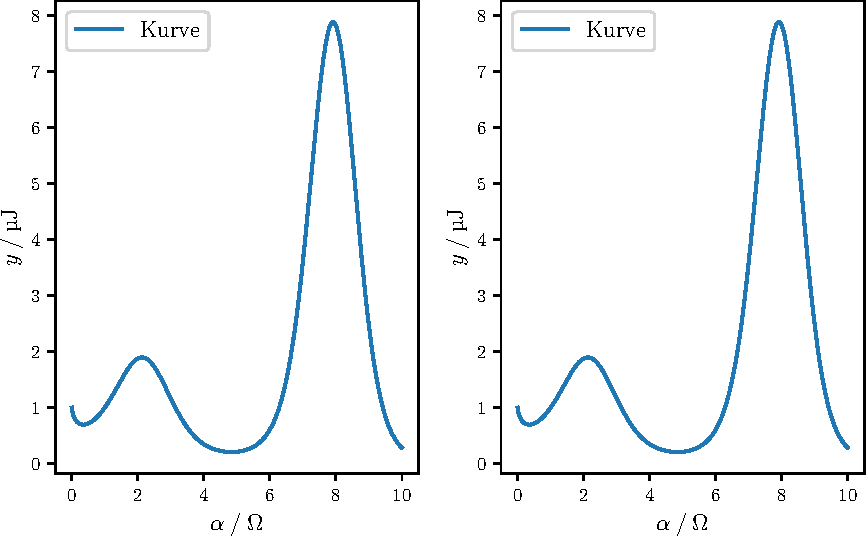
\includegraphics[width=\textwidth]{build/plot.pdf}
    \caption{Grafische Auswertung der Messdaten mit den jeweiligen Theoriekurven.}
    \label{fig:plot}
\end{figure}

\noindent
In \autoref{fig:plot} wurden die Messdaten mit den jeweiligen Theoriekurven grafisch dargestellt. Für die Theoriekurven wurde in die Gleichungen \eqref{eqn:fresnelsenk} und \eqref{eqn:fresnelpara}
ein Literaturwert von
\begin{align*}
    n_{\text{Lit}} = 3,353
\end{align*}
eingesetzt \cite{BrechSilizium}. Die grafische Auswertung liefert näherungsweise einen Brewsterwinkel von  
\begin{align*}
    \alpha_{\text B} = \SI{78}{\degree},
\end{align*}
und daraus ein Brechungsindex von 
\begin{align*}
    \tan(\alpha_{\text B} = \SI{78}{\degree}) = 4,705.
\end{align*}